Une base de données modèlise sommairement le fonctionnement d'un hopital. Les tables et leurs structures sont donnés dans les figures 1 à 9.
\begin{figure}[h]
  \centering
  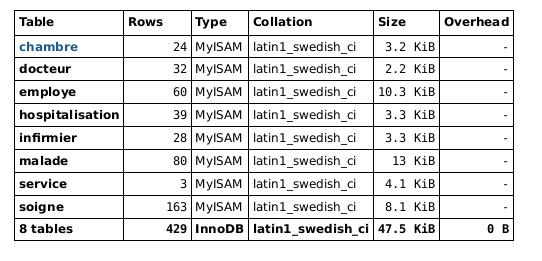
\includegraphics[width=8cm]{./Ehopital_1.png}
  % Ehopital_1.png: 0x0 pixel, 300dpi, 0.00x0.00 cm, bb=
  \caption{Tables (relations) de la base \og hopital\fg.}
  \label{fig:hop_1}
\end{figure}
\begin{figure}
 \centering
 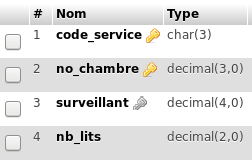
\includegraphics[width=5cm]{./Ehopital_2.png}
 \caption{Chambre}
 \label{fig:hop_2}
\end{figure}
\begin{figure}
 \centering
 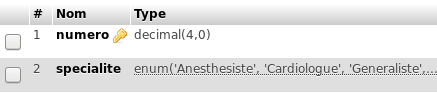
\includegraphics[width=8cm]{./Ehopital_3.png}
 \caption{Docteur}
 \label{fig:hop_3}
\end{figure}
\begin{figure}
 \centering
 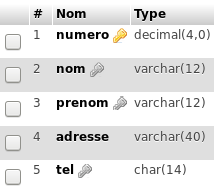
\includegraphics[width=4cm]{./Ehopital_4.png}
 \caption{Employé}
 \label{fig:hop_4}
\end{figure}
\begin{figure}
 \centering
 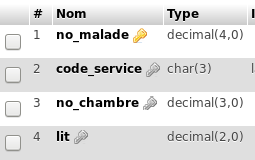
\includegraphics[width=5cm]{./Ehopital_5.png}
 \caption{Hospitalisation}
 \label{fig:hop_5}
\end{figure}
\begin{figure}
 \centering
 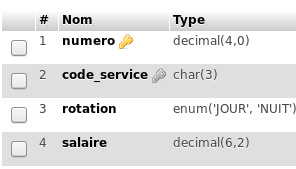
\includegraphics[width=5cm]{./Ehopital_6.png}
 \caption{Infirmier}
 \label{fig:hop_6}
\end{figure}
\begin{figure}
 \centering
 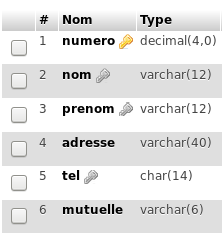
\includegraphics[width=5cm]{./Ehopital_7.png}
 \caption{Malade}
 \label{fig:hop_7}
\end{figure}
\begin{figure}
 \centering
 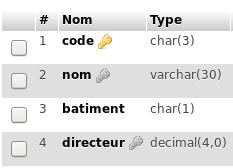
\includegraphics[width=5cm]{./Ehopital_8.png}
 \caption{Service}
 \label{fig:hop_8}
\end{figure}
\begin{figure}
 \centering
 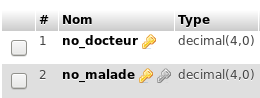
\includegraphics[width=5cm]{./Ehopital_9.png}
 \caption{Soigne}
 \label{fig:hop_9}
\end{figure}


Vous devez coder en SQL les reqêtes suvantes 
\begin{enumerate}
  \item[R1] Prénom et nom de chaque malade affilié à la mutuelle 'MAAF'.
  \item[R2] Prénom et nom des infirmiers(ères) travaillant pendant la rotation de nuit.
  \item[R3] Donner pour chaque service, son nom, son bâtiment, le prénom, le nom et la spécialité de son directeur.
  
  \item[R4] Donner, pour chaque lit du bâtiment 'B' occupé par un patient affilié à une mutuelle dont le nom commence par 'MN...', le numéro du lit dans la chambre, le numéro de la chambre, le nom du service, ainsi que le nom et le prénom du patient ainsi que celui de sa mutuelle.
  
  \item[R5] Quelle est la moyenne des salaires des infirmiers(ères) par service ?
  
  \item[R6] Pour chaque service du bâtiment 'A', quel est le nombre moyen de lit par chambre?
  
  \item[R7] Pour chaque patient soigné par plus de 3 médecins, donner le nombre total de ses médecins ainsi que le nombre de spécialités.
  
  \item[R8] Pour chaque service, quel est le rapporte entre le nombre d'infirmiers(ères) affectés(ées) au service et le nombre de patients hospitalisés dans le service?
  
  \item[R9] Prénom et nom des docteurs soignant au moins un patient hospitalisé.
  
  \item[R10] Prénom et nom des médecins ne soignant aucun patient hospitalisé.
  
  \item[R11] Pour chaque médecin, retrouver le nombre de ses patients hospitalisés, y compris lorsque ce nombre est 0.
  
  \item[R12] Trouver les bâtiments et numéros des chambres occupées par au moins un malade.
  
  \item[R13] Former la liste des identifiants (bâtiment, numeros de chambre) des chambres vides.
  
  \item[R14] Pour chaque chambre, donner le bâtiment, le numéro, le nombre total de lits et le nombre de lits occupés (y compris lorsque ce nombre est 0).
  
  \item[R15] Prénom et nom des médecins ayant un patient hospitalisé dans chaque service.
  
  \item[R16] Prénom et nom des médecins soignant des patients hospitalisés dans toutes les chambres surveillées par l'infirmier nommé 'Roddick'.
  
  \item[R17] Prénom et nom des patients soignés par le directeur du service dans lequel ils sont hospitalisés.
  
  \item[R18] Quelles sont les chambres qui ont des lits disponibles dans le service de cardiologie ?
\end{enumerate}
